\chapter{How to use LELAPE}
\section{Formatting input data}
%
You are supposed to have performed experiments on some memory element. Tests were performed as:
\begin{itemize}
	\item \textbf{Static}: The device was written, sent to standby mode, irradiated and eventually read. The content after the irradiation was compared to the initially writing.
	\item \textbf{Pseudostatic}: Similar to static ones, but standby intervals are shorter than the irradiation time and the memory is read several times during the irradiation. Usually, flipped bits are corrected on the fly \cite{Gupta2017}.
	\item \textbf{Dynamic}: A typical experiment consists in performing a continuous reading \& writing process while the memory is irradiated with a predefined algorithm to detect failures \cite{Tsiligiannis2014a, Tsiligiannis2014b}. 
\end{itemize}

In any of these cases, the researcher saves information about the bitfilps: Word address, read content, initial pattern, ... 
In order to use LELAPE, radiation test data must be converted to a matrix with three or four columns. The meaning of the columns is the following:
\begin{itemize}
	\item \textit{First Column}: Word Address where bitflips were observed.
	\item \textit{Second Column}: Content in the word address after the radiation tests.
	\item \textit{Third Column}: Content in the word address before the irradiation.
	\item \textit{Fourth Column}: In pseudostatic tests, cycle in which the bitflip was observed. This column can be omitted in the static tests or replaced by a column full of ones.  
	
	This calumn is also necessary for dynamic tests. In each step of the algorithm, the memory is fully explored and the discrepancies registered. So, in practice, for analysis with LELAPE the only differences between dynamic and psedostatic tests are that, in the former, the pattern changes from cycle to cycle, and that the addresses are recorded in different orders, sometimes increasing, sometimes decreasing, etc. These details are irrelevant for the tool.
\end{itemize} 

LELAPE needs this elements to be converted to a UInt32 matrix\footnote{In Julia, typing variable is optional but encouraged to speed up calculations.} so it is important that all the elements of the matrix, including the cycle label, are in this format or, at least, in some kind of integer. This makes dangerous labelling the fourth column with words or letters. 

A simple solution consists in grouping the data results in CSV format and read this text file with \texttt{readdlm}, included in the \text{DelimitedFiles} package. In the Jupyter folder, you can see some examples that can guide you to adapt your own data. One advantage of this function is that it can automatically convert the data to the required format, as shown in the Jupyter notebooks.

\section{Setting up the analysis}
%
Before starting the analysis, we must define some additional variables to indicate the software how to proceed. These variables are the followong:
%
\begin{itemize}
	\item \textbf{LA}: Variable in integer format. It indicates the memory size in words (not in bits!). It is often a power of 2.
	\item \textbf{WordWidth}: Also an integer, it indicates the number of bits per word. Typically 8, 16, 32 but other values are possible.
	
	If you had registered your data directly with the cell address, disregarding any organization in words, just set \texttt{WordWidth = 1} and \texttt{LA  = \(L_N\)}, this being the memory size in bits.
	
	\item \textbf{Operation}: A string variable to indicate the mathematical operation used to create the DV set. So far, only two options are implemented:
	\begin{itemize}
		\item \textit{XOR}: Addresses are xored bit to bit. This mode is set with the \texttt{"XOR"} value.
		\item \textit{Positive subtraction}: The absolute value of the difference of addresses is returned. It is marked with \texttt{"POS"}. 
	\end{itemize}

	In practice, we have observed that the former is appropriate for SRAMs and the latter for FPGAs. However, this idea may be erroneous due to the use of few and partial radiation test data.
	%
	\item \textbf{UsePseudoAddress}: The pseudoaddress is defined as follows: let us suppose that we have observed a bitflip in the $k$-th position of the $NWA$-th word address, The word width is $W$ and $k=0$ corresponds to the least significant bit, $W-1$ to the most significant one. Hence, the pseudoaddress of the bitflip is:
	%
	\begin{equation}
		PSA = NWA \cdot W + k
		\label{Eq:PseudoAddress}
	\end{equation}
	%
	This value is full of meaning in FPGAs since just returns the position of the cell in the bitflips. It is completly artificial in some SRAMs but somehow analysis using the pseudoaddress instead of the word address are more accurate and efficient. 
	
	The researcher can set this variable to \texttt{true} or \texttt{false} at will.
	%
	\item \textbf{KeepCycles}: In pseudostatic tests, this boolean variable indicates that the system must use the information about the cycles (fourth column) or just using the set of data as a whole. 
	
	Before going on, a little tip to treat data from\textbf{ field tests} where a large number of similar devices are exposed to natural radiation. An option to analyze data would have been define a new pseudoaddress adding the position of the device in the bank, \(k_{MEM}\), and the memory size in bits, \(L_N\):
	\[
		PSA^* = k_{MEM}\cdot L_N + NWA \cdot W + k
	\]
	This may work, but is strongly computationally inefficient for LELAPE. Instead of it, we recommend to redefine the reading cycle index. Let us suppose that there are \(N_{MEM}\) identical memories in the bank, and that they are indexed from \(k_{MEM}=0\) to \(k_{MEM}=N_{MEM}-1\). If the bank reading cycle is \(k_{BNK}\), the cycle to be included in the CSV file should be:
	%
	\begin{equation}
		Cycle = k_{BNK}\cdot N_{MEM}+k_{MEM}
	\end{equation}
	%
	In other words, we are redefining cycles at device level, not bank level. This solution is much more efficient for LELAPE.
	%
	\item \textbf{TraceRuleLength}: This an integer variable with 1,2 or 3 as allowed values. LELAPE looks for anomalously repeated elements in the DV set with very few ones in binary representation. The user can decide if looks for elements with 1, 2 or 3 ones or less and include them as candidates to detect pairs. 
	%
	\item \textbf{$\varepsilon$}: A float number always positive but close to 0. If the expected number of elements repeated $k$ times in the DV set is lower than $\varepsilon$, we must consider this number of repetitions impossible. If higher, we determine than at least an element can appear $k$ times just due to randomness. Default value is 0.05.
	
	A very low value of $\varepsilon$ will exclude false positive but also genuine values relating pair of addresses in an MCU. On the contrary, if it is chosen too low, false positives might be taken as good ones.
	%
	\item \textbf{LargestMCUSize}: During the search of critical DV values, LELAPE starts to group addresses in provisional MCUs that grow large and large as new possible critical DV values are tested. Unfortunately, sometimes this process does not find a stable solution and goes on looking for it despite being unrealistic. This parameter is used to stop the calculation since it informs the software of not considering MCUs with more than \textit{LargestMCUSize} addresses. By default, it is set to 200, but, if you do not expect such a large event, reduce its value in order to unburden the computer memory usage. 
\end{itemize}

 \section{Functions in the module}
 %
 The functions depicted in this section are included in LELAPE and also accessible from the REPL, Jupyter, etc. Other functions are for internal use in LELAPE and are excluded from this list. The reader can just open the individual \texttt{.jl} files and check the comments.
 
 Available functions are grouped in several categories:
 \begin{itemize}
 	\item \hyperref[SubseC:PreparationExpdata]{Preparation of experimental data}
 	\item \hyperref[SubSeC:MBUs]{Multiple Bit Upsets}
 	\item \hyperref[Subsec:StatisticalPredictions]{Statistical predictions}
 	\item \hyperref[Subsec:SearchOfAnomalies]{Search of anomalies}
 	\item \hyperref [SubSec:ClassificationEventsFromAnomalies]{Classification of events from anomalies}
 	\item \hyperref[SubSec:FalseEvents]{False events due to accumulation of bitflips}
 \end{itemize}
 %
 In all the items you will find the accepted input arguments, the kind of output as well as an explication of its purpose.
 %
 \subsection{Preparation of experimental data}\label{SubseC:PreparationExpdata}
 %
 These functions just adapt the original test data to be used by LELAPE, or provide information about the data set. In this section, the following functions are included:
 \begin{itemize}
 	\item \hyperref[Func:ConvertToPseudoADD]{ConvertToPseudoADD}
 	\item \hyperref[Func:AddPatternColumn]{AddPatternColumn}
 	\item \hyperref[Func:ExtractFlippedBits]{ExtractFlippedBits}
 	\item \hyperref[Func:Npairs]{Npairs}
 	\item \hyperref[Func:NTriplets]{NTriplets}
 \end{itemize}
 %
 \subsubsection*{ConvertToPseudoADD}\label{Func:ConvertToPseudoADD}
 \begin{itemize}
 	\item \textbf{Input arguments}: 
 	\begin{itemize}
 		\item \textit{Method 1: }\textbf{DATA}::Array\{UInt32\}, \textbf{WordWidth}::Int
 		\item \textit{Method 2: }\textbf{DATA}::Array\{UInt32\}, \textbf{WordWidth}::Int, \textbf{KeepCycle}::Bool
 	\end{itemize}
 
 	In the case of not providing \textbf{KeepCycle}, it is assumed to be \texttt{false}.
 
 	\item   \textbf{Output}: Array\{UInt32, 2\}, or Matrix\{UInt32\}.
 	\item  This function looks for the flipped bits between words in the same row but in the second
 	and third columns of the \textbf{DATA} matrix. It does not matter if there are several bitflips, since they are independently counted. 
 	The pseudoaddress  of each bitflip, defined as \[\text{WORDADDRESS}\times\text{Wordwith}+\text{Bitposition}\] (Eq. \ref{Eq:PseudoAddressDefinition}) is returned as the first column of the output.
 
 	If there is information about the different cycles, it can be kept in the optional second column in the output with the condition of previously declaring \textbf{KeepCycle} as true. If cycle information is absent, the second column is filled with 1's.
 	
 	Fig. \ref{fig:Example_ConvertToPseudoADD} shows an example of use in the REPL. There are more rows in the output matrix than in the input one since there are words with several flipped bits.
 	
 	\begin{figure}[h!]
 		\centering
 		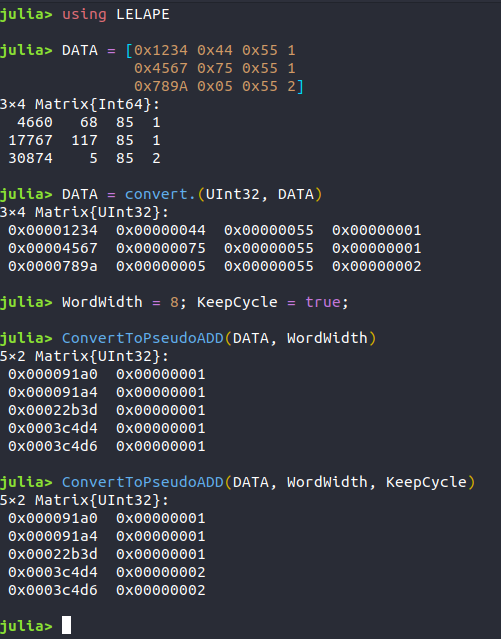
\includegraphics[width=0.65\columnwidth]{fig/functions/ConvertToPsudoADD.png}
 		\caption{Example of use of \texttt{ConvertToPseudoADD}.}
 		\label{fig:Example_ConvertToPseudoADD}
 	\end{figure}
 \end{itemize}
%
 \subsubsection*{AddPatternColumn}\label{Func:AddPatternColumn}
 
  \begin{itemize}
 	\item \textbf{Input arguments}: 
 	\begin{itemize}
 		\item \textit{Method 1: }\textbf{DATA}::Matrix\{UInt32\}, \textbf{PATTERN}::UInt32
 		\item \textit{Method 2: }\textbf{DATA}::Matrix\{UInt32\}, \textbf{PATTERN}::UInt16
 		\item \textit{Method 3: }\textbf{DATA}::Matrix\{UInt32\}, \textbf{PATTERN}::UInt8
 	\end{itemize}
 
 	\textbf{DATA} must have 2 or 3 columns, as explained later. If the matrix does not accomplish this condition, the function returns an error.
 
 	\item \textbf{Output}: Matrix{UInt32}
 	\item     Sometimes, \textbf{DATA} are just a matrix with only two columns: \textit{Word Address} \& \textit{Content}, assuming that the PATTERN is constant. This function just expands the matrix
 	to include a column in the third position with the used \textbf{PATTERN}. 
 	
 	Sometimes, in pseudostatic tests, there is a third column with cycle information. In this case, this column is shifted to the fourth position, and the void third column filled with the \textbf{PATTERN}. 
 	 %
 	\begin{figure}[h!]
 		\centering
 		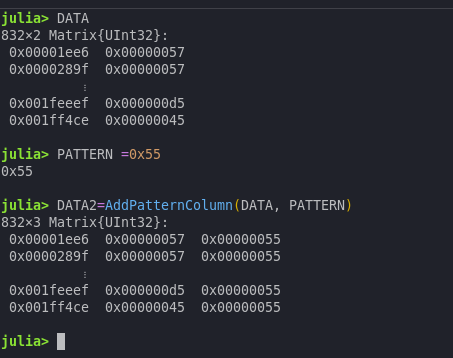
\includegraphics[width=0.65\columnwidth]{fig/functions/AddPatternColumn.png}
 		\caption{Example of use of \texttt{AddPatternColumn}.}
 		\label{fig:Example_AddPatternColumn}
 	\end{figure}
 
 	Fig. \ref{fig:Example_AddPatternColumn} shows an example of use of this function for a simple case.
 
 \end{itemize}
 
 \subsubsection*{ExtractFlippedBits}\label{Func:ExtractFlippedBits}
 \begin {itemize}
 \item \textbf{Input arguments}:
 \begin{itemize}
 	\item \textit{Method 1: }\textbf{WORD}::UInt32, \textbf{PATTERN}::UInt32, \textbf{Wordwidth}::Int
 	\item \textit{Method 2: }\textbf{WORD}::UInt16, \textbf{PATTERN}::UInt16, \textbf{Wordwidth}::Int
 	\item \textit{Method 3: }\textbf{WORD}::UInt8, \textbf{PATTERN}::UInt8, \textbf{Wordwidth}::Int
 \end{itemize}
 \item \textbf{Output}: :Array\{Int,1\}, or Vector\{Int\}
 \item This function allows discovering the position of different bits between \textbf{WORD}
 and \textbf{PATTERN}. It also verifies that both values are coherent with the \textbf{Wordwidth},
 meaning that neither of them are higher than \(2^{Wordwidth}-1\). A vector, never larger than \textbf{Wordwidth} is returned. If this condition is not fulfilled, the functions returns an error. If \textbf{WORD} and \textbf{PATTERN} are equal, the output is a void vector.
 %
 \begin{figure}[h!]
 	\centering
 	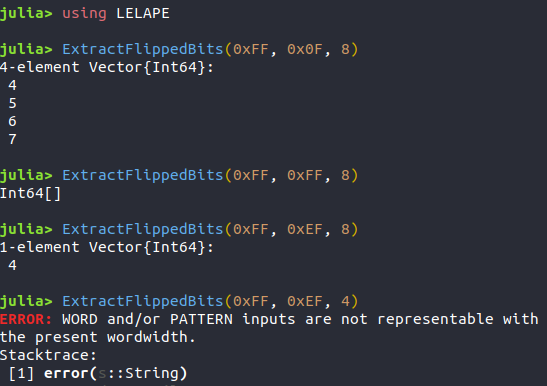
\includegraphics[width=0.65\columnwidth]{fig/functions/ExtractFlippedBits.png}
 	\caption{Example of use of \texttt{ExtractFlippedBits}.}
 	\label{fig:Example_ExtractFlippedBits}
 \end{figure}
 
 Fig. \ref{fig:Example_ExtractFlippedBits} shows some examples of use of this function. Take into account that, even when there is a single bitflip, a vector is always returned, albeit with an only value inside.
\end{itemize}
%
\subsubsection*{NPairs}\label{Func:Npairs}
\begin{itemize}
	\item \textbf{Input arguments}:
	\begin{itemize}
		\item \textit{Method 1}: \textbf{DATA}::Array{UInt32}
		\item \textit{Method 2}: \textbf{DATA}::Array{UInt32}, \textbf{UsePseudoAdd}::Bool
		\item \textit{Method 3}: \textbf{DATA}:: Array{UInt32}, \textbf{UsePseudoAdd}::Bool, \textbf{WordWidth}:: Int
		\item \textit{Method 4}: \textbf{DATA}::Array{UInt32}, \textbf{UsePseudoAdd}:: Bool, \textbf{WordWidth}:: Int, \textbf{KeepCycle}:: Bool
		\item \textit{Method 5}: \textbf{N}::Int
	\end{itemize}

	In Methods 1--4, default values for parameters are \texttt{\textbf{UsePseudoAdd} = false}, \texttt{\textbf{WordWidth} = 1}, \texttt{\textbf{KeepCycle} = false}. 
	
	\item \textbf{Output}: Int 
	%
	\item \textbf{DATA} is a 3 or 4-column matrix derived from the loaded CSV file and each row containing the word address (\#1), the read word after the tests (\#2), the initial pattern (\#3) and the number of reading cycle when the error was observed. If this last column is not provided or \textbf{KeepCycle} is false, the system works as if only one cycle was done. 
	
	The function provides the number of pairs of addresses taken during each cycle regarding predictions of the Only-SBU model (Eq. \ref{Eq:SizeOfDV}). For example, let us suppose that we have done 2 cycles, observing in the first one 30 events, and 40 in the second. The number of possible pairs is the addition of the pairs in each cycle:
	\[
	\frac{1}{2}\cdot 30\cdot(30-1)+\frac{1}{2}\cdot 40\cdot(40-1) = 1215
	\]
	Thus, 1215 pairs can be formed. If we had not taken into account the existence of cycles, the number of pairs would have been\[	\frac{1}{2}\cdot (30+40)\cdot(30+40-1) = 2415\]
	however, many of them are unreal since were taken in different times!
	
	If \textbf{UsePseudoAdd} is set to true, the system looks for the position of the bitflips inside the word and uses the pseudoaddress (\(\text{WordAddress}\times\text{WordWidth}+\text{Position}\)). Thus, it is necessary to provide the \textbf{WordWidth} value (8, 16, 32, ...). Using \textbf{DATA} as the only argument is appropriate to analyze values directly in pseudoaddress format (or just the word address) taken during one only cycle. This is the case, for example, of FPGAs configuration memory. 
	
	There is a final method, just saying the number of observed pairs, \textbf{N}. In this case, the function returns \textbf{N}\(\cdot\)(\textbf{N}-1)/2.

	\begin{figure}[h!]
		\centering
		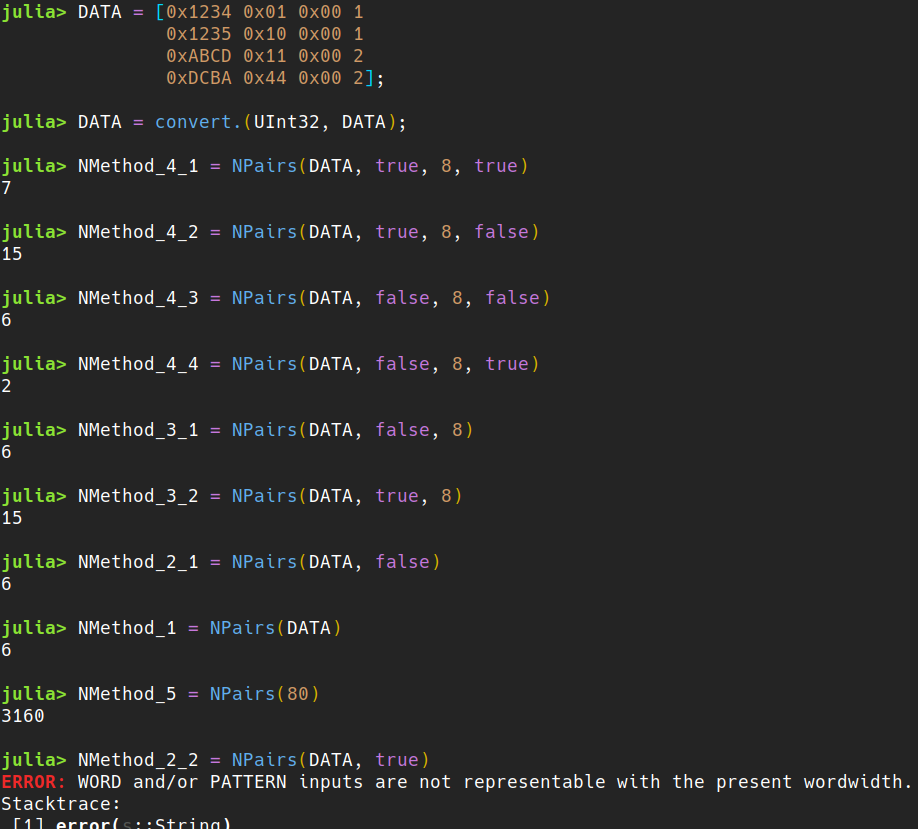
\includegraphics[width=0.75\columnwidth]{fig/functions/NPairs.png}
		\caption{Example of use of \texttt{NPairs}.}
		\label{fig:Example_NPAirs}
	\end{figure}

	Fig. \ref{fig:Example_NPAirs} shows an example of use of this function. 
	
\end{itemize}
%
\subsubsection*{NTriplets}\label{Func:NTriplets}
\begin{itemize}
	\item \textbf{Input arguments}:
	\begin{itemize}
		\item \textit{Method 1}: \textbf{DATA}::Array{UInt32}
		\item \textit{Method 2}: \textbf{DATA}::Array{UInt32}, \textbf{UsePseudoAdd}::Bool
		\item \textit{Method 3}: \textbf{DATA}:: Array{UInt32}, \textbf{UsePseudoAdd}::Bool, \textbf{WordWidth}:: Int
		\item \textit{Method 4}: \textbf{DATA}::Array{UInt32}, \textbf{UsePseudoAdd}:: Bool, \textbf{WordWidth}:: Int, \textbf{KeepCycle}:: Bool
		\item \textit{Method 5}: \textbf{N}::Int
	\end{itemize}
	\item \textbf{Output}: Int
	%
	\item Similar to \textit{Npairs(...)}, but calculating the expected number of triplets instead of pairs. Thus, instead of using Eq. \ref{Eq:SizeOfDV} as the basis for calculations, this function uses:
	\[
		N_{Triplets} = \frac{1}{6}\cdot N_{BF}\cdot \left(N_{BF}-1\right)\cdot \left(N_{BF}-2\right)
	\]
\end{itemize}
%
\subsection{Multiple Bit Upsets} \label{SubSeC:MBUs}
%
Sometimes, the researcher just wants to know how many multiple bit upsets occurred during the experiments. There is only one function in this section, \texttt{CheckMBUs}.

\subsubsection*{CheckMBUs}

\begin{itemize}
	\item \textbf{Input arguments}:
	\begin{itemize}
		\item \textit{Method 1}: \textbf{WORD}::UInt32, \textbf{PATTERN}::UInt32, \textbf{WordWidth}::Int
		\item \textit{Method 2}: \textbf{WORDS}::Vector\{UInt32\}, \textbf{PATTERN}::Vector\{UInt32\}, \textbf{WordWidth}::Int
		\item \textit{Method 3}:  \textbf{WORDS}::Vector\{UInt32\}, \textbf{PATTERN}::UInt32, \textbf{WordWidth}::Int
	\end{itemize}
	\item \textbf{Output}: 
		\begin{itemize}
			\item \textit{Method 1}: Tuple\{Int, Vector\{Int\}\}
			\item \textit{Methods 2 \& 3}: Tuple\{Vector\{Int\}, Vector\{Any\}\}
		\end{itemize}
	%
	\item The first method is quite easy to understad. It just takes to unsigned integer 32-bit numbers, \textbf{WORD} \& \textbf{PATTERN}, of which only the last \textbf{WordWidth} bits are significant, and looks for equivalent bits with different value with the function \hyperref[Func:ExtractFlippedBits]{\texttt{ExtractFlippedBits}}. Then, it returns the number of biflips and a vector containing the flipped positions. Fig. \ref{fig:Example_CheckMBUs_M1} shows how this function behaves with these inputs.
	
	\begin{figure}[h!]
		\centering
		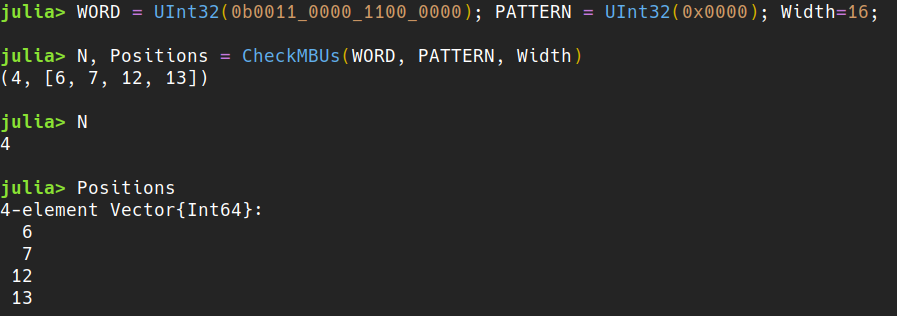
\includegraphics[width=0.75\columnwidth]{fig/functions/CheckMBUs_M1.png}
		\caption{Example of use of \texttt{CheckMBUs} with unsigned integers as inputs.}
		\label{fig:Example_CheckMBUs_M1}
	\end{figure}

	For Method 2, the idea is to provide as arguments two similar-length vectors with the \textbf{WORD} and \textbf{PATTERN} values in UInt32 format, as well as the \textbf{WordWidth}. Then, the function checks the values in both vectors with the same index and returns two vectors. The first one is a typical vector of integers, containing in the \(k\)-th position the number of different bits between \textbf{WORD}[k] y \textbf{PATTERN}[k]. The second is a vector of vectors. Thus, the element in the \(k\)-th positiion is also a vector with the positions of the flipped bits. 
	
	Method 3 is quite similar to Method 2, but \textbf{PATTERN} is no longer a vector but a constant value for all the elements of \textbf{WORDS}. Fig. \ref{fig:Example_CheckMBUs_M23} shows how this method and the previous one work.
	
	\begin{figure}[h!]
		\centering
		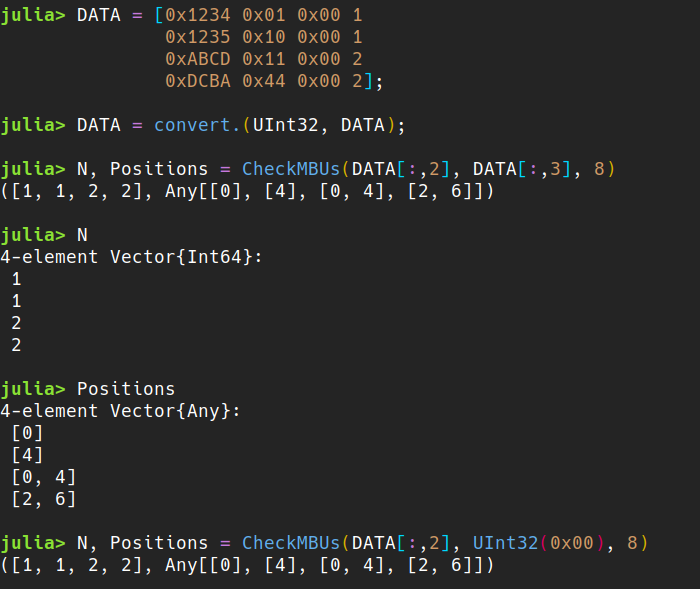
\includegraphics[width=0.75\columnwidth]{fig/functions/CheckMBUs_Methods2_3.png}
		\caption{Example of use of \texttt{CheckMBUs} with vectors as inputs. Last line uses Method 3, where the pattern is provided as an unsigned integer.}
		\label{fig:Example_CheckMBUs_M23}
	\end{figure}
	
\end{itemize}
%
\subsection{Statistical predictions}\label{Subsec:StatisticalPredictions}
%
The goals of this set of functions is to cast predictions about the characteristics of the data according to the Only-SBU model. The following functions are included in this section:

\begin{itemize}
	\item \hyperref[Subsec:MaxExpectedRepetitions]{MaxExpectedRepetitions}
	\item \hyperref[Subsec:TheoAbundance_POS]{TheoAbundance\_POS}
	\item \hyperref[Subsec:TheoAbundance_XOR]{TheoAbundance\_XOR}
	\item \hyperref[Subsec:TheoAbundance]{TheoAbundance}
\end{itemize}

Related to these functions are those used to determine the expected number of false errors, but they will be depicted in the corresponding section.
%
\subsubsection*{MaxExpectedRepetitions}\label{Subsec:MaxExpectedRepetitions}
%
\begin{itemize}
	\item \textbf{Input arguments}: 
	\begin{itemize}
		\item \textit{Method 1}: \textbf{NDV}::Int, \textbf{LN}::Int, \textbf{Operation}:: String, \(\varepsilon\):: AbstractFloat	
		\item \textit{Method 2}: \textbf{NDV}::Int, \textbf{LN}::Int, \textbf{Operation}::String
	\end{itemize}
	\item \textbf{Output}: Int
	\item The purpose of this funcion is to determine the maximum number of expected
	repetitions. in a DV set taken from a memory with size equal to \textbf{LN} .
	In general, it is the first integer such that its theoretical abundance is
	lower than \(\varepsilon\). If this threshold is not provided, it is assumed to be \(\varepsilon = 0.01\).
\end{itemize}
%
\subsubsection*{TheoAbundance\_POS}\label{Subsec:TheoAbundance_POS}
%
\begin{itemize}
	\item \textbf{Input arguments}:
	%
	\begin{itemize}
		\item \textit{Method 1}: \textbf{NR}: :Int, \textbf{NB}::Int, \textbf{LN}::Int, \textbf{UsingDV}::Bool
		\item \textit{Method 2}: \textbf{NR}: :Int, \textbf{NB}::Int, \textbf{LN}::Int
	\end{itemize}
	\item \textbf{Output:} AbstractFloat
	%
	\item This function allows calculating the expected number of values repeated 	 \textbf{NR} times after several bitflips in a memory with \textbf{LA} words with \textbf{W} bits per word   	supposing to have used the POSITIVE subtraction.
	
	\textbf{NR} must be an integer number higher than or equal to 0. 
	\textbf{NB} is an integer number supposed to be higher than 1.
	\textbf{LN} is an integer number, and indicates the size of the memory. If the researcher uses bit address for calculations, \textbf{LN} is \textbf{LA}\(\times\)\textbf{W}. However, if he/she uses the word address instead, this parameerter is \textbf{LA}.
	
	\textbf{UsingDV} determines how \textbf{NB} must be interpreted. If that boolean variable is \texttt{true}, \textbf{NB} is the size of the DV set, called elsewhere \(N_{DV}\). If false, \textbf{NB} is the number of bitflips and \(N_{DV}\) must be calculated from it. By default, \textbf{UsingDV} is \texttt{false}.
	
	Equations were got from Eq.2 of the Appendix in J. C. Fabero et al., "\textit{Single Event Upsets Under 14-MeV Neutrons in a 28-nm
		SRAM-Based FPGA in Static Mode,}" in IEEE Transactions on Nuclear Science, vol.
	67, no. 7, pp. 1461-1469, July 2020, doi: 10.1109/TNS.2020.2977874.
	
	Lawfully avalaible for free download on \href{https://eprints.ucm.es/id/eprint/59496/}{https://eprints.ucm.es/id/eprint/59496/}
\end{itemize}

\subsubsection*{TheoAbundance\_XOR}\label{Subsec:TheoAbundance_XOR}
%
\begin{itemize}
	\item \textbf{Arguments:}
	%
	\begin{itemize}
		\item \textit{Method 1}: \textbf{NR}: :Int, \textbf{NB}::Int, \textbf{LN}::Int, \textbf{UsingDV}::Bool
		\item \textit{Method 2}: \textbf{NR}: :Int, \textbf{NB}::Int, \textbf{LN}::Int
	\end{itemize}
	\item \textbf{Output:} AbstractFloat
	%
	\item Equivalent to \hyperref[Subsec:TheoAbundance_POS]{\texttt{TheoAbundance\_POS}}, but referred to the bitwise XOR operation. 
	
	Equations were got from Eq.12 of the Appendix.C in 
	F. J. Franco et al., "\textit{Statistical Deviations From the Theoretical Only-SBU
		Model to Estimate MCU Rates in SRAMs,}" in IEEE Transactions on Nuclear
	Science, vol. 64, no. 8, pp. 2152-2160, Aug. 2017,
	doi: 10.1109/TNS.2017.2726938. 
	
	Lawfully avalaible for free on https://eprints.ucm.es/id/eprint/43874/
\end{itemize}
%
\subsubsection*{TheoAbundance}\label{Subsec:TheoAbundance}
%
\begin{itemize}
	\item \textbf{Input arguments}:
	\begin{itemize}
		\item \textit{Method 1:} \textbf{NR}::Int, \textbf{NB}::Int, \textbf{LN}::Int, \textbf{Operation}:: String, \textbf{UsingDV}::Bool
		\item \textit{Method 1:} \textbf{NR}::Int, \textbf{NB}::Int, \textbf{LN}::Int, \textbf{Operation}:: String
	\end{itemize}
	\item \textbf{Output}: AbstractFloat
	\item This is an Alias for \hyperref[Subsec:TheoAbundance_POS]{ \texttt{TheoAbundance\_POS()}} or \hyperref[Subsec:TheoAbundance_XOR]{ \texttt{TheoAbundance\_XOR()}}. The definition of arguments are similar, with an additional parameter, \textbf{Operation}, which only can be \texttt{"XOR"} or \texttt{"POS"}. 
	
\end{itemize}
%%

%%%%%%%%%%%%%%%%%%%%%%%%5
\subsection{Search of anomalies}\label{Subsec:SearchOfAnomalies}

This is an important set of functions that determine the statistical anomalies in the data set, and discard those that are not trustworthy, perhaps due to interaction between events. 

The functions included in this section are:

\begin{itemize}
	\item  \hyperref[Fun:DetectAnomaliesSelfConsis]{DetectAnomalies\_SelfConsis}
	\item  \hyperref[Fun:DetectAnomaliesShuffleRule]{DetectAnomalies\_Shuffle\_Rule}
	\item  \hyperref[Fun:DetectAnomaliesTraceRule]{DetectAnomalies\_Trace\_Rule}
	\item  \hyperref[Fun:DetectAnomaliesMCURule]{DetectAnomalies\_MCU\_Rule}
	\item  \hyperref[Fun:DetectAnomaliesFullCheck]{DetectAnomalies\_FullCheck}
\end{itemize}

Last function just calls the previous four.

\subsubsection*{DetectAnomalies\_SelfConsis}\label{Fun:DetectAnomaliesSelfConsis}
\begin{itemize}
	\item \textbf{Input arguments}:
	\begin{itemize}
		\item  \textit{Method 1: }\textbf{DATA}::Array\{UInt32, 2\}, 
		\textbf{WordWidth}::Int,
		\textbf{LN0}::Int,
		\textbf{Operation}::String,
		\textbf{UsePseudoADD}::Bool,
		\textbf{KeepCycle}::Bool,
		\textbf{\(\varepsilon\)}::AbstractFloat,
		\textbf{LargestMCUSize}::Int
		%
		\item  \textit{Method 2: }\textbf{DATA}::Array\{UInt32, 2\}, 
		\textbf{WordWidth}::Int,
		\textbf{LN0}::Int,
		\textbf{Operation}::String,
		\textbf{UsePseudoADD}::Bool,
		\textbf{KeepCycle}::Bool,
		\textbf{\(\varepsilon\)}::AbstractFloat
		%
		\item  \textit{Method 3: }\textbf{DATA}::Array{UInt32, 2}, 
		\textbf{WordWidth}::Int,
		\textbf{LN0}::Int,
		\textbf{Operation}::String,
		\textbf{UsePseudoADD}::Bool,
		\textbf{KeepCycle}::Bool
	\end{itemize}

	Default values for \textbf{\(\varepsilon\)} \& 	\textbf{LargestMCUSize} are \texttt{0.05} and \texttt{200} respectively.
	%
	\item \textbf{Output: } Array\{UInt32, 2\}	
	%
	\item This function will calculate the anomalies in the set of addresses using \hyperref[Subsec:SelfConsistencyRule]{the Self Consistency rule}. 
	 First of all, let us know the inputs:
	 \begin{itemize}
	
		\item   \textbf{DATA}: A matrix with 3 or 4 columns. 
			 \begin{itemize}
			 	\item The first column contains the word addresses in UInt32 format.
			 	\item The second one shows the content read in the memory after the irradiation.
			 	\item The third one, the pattern that should be inside.
			 	\item  The fourth one is optional and shows the number of the read cycle if the   memory was read and corrected several times during the irradiation.
			 \end{itemize}
		\item   \textbf{WordWidth}: The size of each word in bits, usually 8, 16. 32, etc. No default value is provided.
		\item   \textbf{LN0}: The memory size in words (not in bits!!!). In many cases, a natural power of 2.
		\item   \textbf{Operation}: A string variable to indicate the preferred operation to calculate
	    the DV set. Only two operations are allowed: 
	    \begin{itemize}
	    	\item \texttt{"XOR"}: bitwise XOR.
	    	\item\texttt{ "POS"}: positive subtraction
	    \end{itemize}
		\item  \textbf{UsePseudoADD}: A boolean variable. Its purpose is to indicate that the user wants to use the word addresses when this parameter is false). If true, the pseudoaddress, calculated
	    as \(\text{WORADDRESS}\times\text{WordWidth} + \text{BitPosition}\), is used instead. Full of sense in FPGA since it is just the position  of the bit in the bitstream, it has not physical interpretation in memories BUT works!!!!
		\item   \textbf{KeepCycle}: If true, the function looks for the fourth column and uses it to calculate the DV Set.
		\item   \textbf{\(\varepsilon\)}: A small positive integer number to determine the threshold that defines when a number of repetitions are impossible to occur. Set by default to 0.05 if not provided among the input arguments.
		\item  \textbf{LargestMCUSize}: This value indicates the largest possible size for MCUs. It has not physical sense  and is only used to stop the program if unrealistic events occur. Set to 200 if not given as an input.

	\end{itemize}
	
	The function returns an \(N\times 2\) UInt32 matrix. The first column contains the anomalously repeated values of the DV SET compatible with the Self Consistency test. The second one contains the number of times they appear in the DV set. Due to format integrity reasons, this column is expressed in unnatural \texttt{UInt32} format. 
	
	It is advisable a latter conversion into Int to make this column more readable. There are several examples of this function or equivalent in the Jupyter folder.
	
	If the function does not find any anomaly, it returns a void matrix.  Or, more exactly, a \(0\times 2\) one.
\end{itemize}
%
\subsubsection*{DetectAnomalies\_Shuffle\_Rule}\label{Fun:DetectAnomaliesShuffleRule}
 TBD
 %
 \subsubsection*{DetectAnomalies\_Trace\_Rule}\label{Fun:DetectAnomaliesTraceRule}
 %
 TBD
 %
 \subsubsection*{DetectAnomalies\_MCU\_Rule}\label{Fun:DetectAnomaliesMCURule}
 %
 TBD
 %
 \subsubsection*{DetectAnomalies\_FullCheck}\label{Fun:DetectAnomaliesFullCheck}
 %
 TBD
 %
 \subsection{Classification of events from anomalies}\label{SubSec:ClassificationEventsFromAnomalies}
 \subsubsection*{MCU\_Indexes}
 %
 \begin{itemize}
 	\item \textbf{Input arguments}: 
 		\begin{itemize}
 			\item \textit{Method 1: } \textbf{DATA}::Matrix\{UInt32\}, 
 			\textbf{OPERATION}::String,
 			\textbf{Markers}:: Vector\{UInt32\}, 
 			\textbf{UsePseudoADD}::Bool, 
 			\textbf{WordWidth}::Int,
 			\textbf{LimitMCUSize}:: Int
 			%
 			\item \textit{Method 2: } \textbf{DATA}::Matrix\{UInt32\}, 
 			\textbf{OPERATION}::String,
 			\textbf{Markers}:: Vector\{UInt32\}, 
 			\textbf{UsePseudoADD}::Bool, 
 			\textbf{WordWidth}::Int
 			%
 			\item \textit{Method 3: } \textbf{DATA}:Matrix\{UInt32\}, 
 			\textbf{OPERATION}::String,
 			\textbf{Markers}:: Vector\{UInt32\}, 
 			\textbf{UsePseudoADD}::Bool
 			%
 			\item \textit{Method 4: } \textbf{DATA}::Matrix\{UInt32\}, 
 			\textbf{OPERATION}::String,
 			\textbf{Markers}:: Vector\{UInt32\}, 
 		\end{itemize}
 	\item \textbf{Output}: Matrix\{Int\}
 	%
 	\item This functions uses the \textbf{DATA} set to look for pairs of addresses which treated with 	 \textbf{OPERATION} yield one of the \textbf{MARKERS}. If an \textbf{ADDRESS} is related to other two addresses, 	 a 3--bit MCU appears (and so on.) The rest of parameters are used to provide necessary  information to use the \textbf{PSEUDOADDRESS} instead of the \textbf{WORD ADDRESS}. 
	 
	 More information about the inputs:
	 
	 \begin{itemize}
	 	\item DATA: A matrix with 3 or 4 columns. 
	 		\begin{itemize}
	 			\item  The first one contains the word addresses in UInt32 formata.
	 			\item        The second one shows the content read in the memory after the irradiation.
	 			\item        The third one, the pattern that should be inside.
	 			\item        The fourth one is optional and shows the namber of the read cycle if the  memory was read and corrected several times during the irradiation.
	 		\end{itemize}
	 	%       
	 	\item \textbf{OPERATION}: A string variable to indicate the preferred operation to calculate
	 	the DVSET. Only two operations are allowed: 
	 	\begin{itemize}
	 		\item "XOR": XORing bit to bit.
	 		\item "POS": abs(a-b)
	 	\end{itemize}
	 	%
	 	\item \textbf{UsePseudoADD}: A boolean variable. It allows to indicate that the user wants to user
	 	word addresses (false). If true, a pseudoaddress is assigned to each bit and calculated
	 	as \[\text{WORDADDRESS}\times\text{WordWidth} + \text{BitPosition.}\] Full of sense in FPGA since it is just the position
	 	of the bit in the bitstream, it has not physical interpretation in memories BUT works!!!!
	 	%
	 	\item \textbf{WordWidth}: The size of each word in bits, usually 8, 16. 32, etc.
	 	%
	 	\item \textbf{LargestMCUSize}: This value indicates the largest possible size for MCUs. It has not physical sense
	 	and is only used to stop the program if unreallistic events occur. Initially set to 200.
	 \end{itemize}
  
	 Concerning the OUTPUT: It provides an integer NMCU\(\times\)LMCU matrix, NMCU being the number of detected MCUs and
	 LMCU the size of the largest reconstructed MCU. Every value different than 0 must be determined as follows:
	 \begin{enumerate}
	 	\item UsePseudoADD = false: The index indicates the row in DATA with the address in the MCU.
	 	\item UsePseudoADD = true: It provides the index in the PSEUDOADDRESS derived SET. If the exact position of
	 	the bitcell is required, DATA should be treated with ConvertToPseudoADD() and
	 	the index used in the resulting matrix.
	 \end{enumerate}
 
     In both cases, if the size of the MCU is smaller than LMCU, the row will be filled with zeros until
     reaching the desired length. For example, if the content of a row is [5 7 9 0 0], it must be interpreted
     as a 3-bit MCU involving addresses indexed with 5, 7 \& 9 in an experiment in which at least a 5-bit 
     MCU (and nothing larger) was observed.
     
 	Finally, if the index of an address does not appear in the returned matrix, it should be interpreted as  isolated and belonging to an SBU.
 	
 \end{itemize}
%
\subsubsection*{Classify\_Addresses\_in\_MCU}
%
\begin{itemize}
	\item \textbf{Input arguments}: 
		\begin{itemize}
			\item \textit{Method 1}: \textbf{DATA}:: Matrix\{UInt32\}, 
			\textbf{Indexes}:: Matrix\{Int\}, 
			\textbf{UsePseudoADD}:: Bool, 
			\textbf{WordWidth}:: Int
			%
			\item \textit{Method 2}: \textbf{DATA}:: Matrix\{UInt32\}, 
			\textbf{Indexes}:: Matrix\{Int\}, 
			\textbf{UsePseudoADD}:: Bool 
			%
			\item \textit{Method 3}: \textbf{DATA}:: Matrix\{UInt32\}, 
			\textbf{Indexes}:: Matrix\{Int\}
		\end{itemize}
	%
	\item \textbf{Output}: Vector:: \{Any\}
	%
	\item The purpose of this function is to classify the addresses (or pseudoaddresses) with bitflips transform the matrix of INDEXES got from MCU\_Indexes() into a Vector of matrices, called SOLUTION, which is eventually returned as OUTPUT.
	 
	The length of SOLUTION is the size of the largest observed MCU(s), NLMCU. Thus, SOLUTION[1] is 	a N x NLMCU matrix in which every row contains the addresses or pseudoaddresses of the NLMCU 	bitflips involved in this MCU. N is the number of observdd NLMCU-bit MCUs.
	
	SOLUTION[2] is devoted to events with M = NLMCU-1 bits. As before, it is a matrix with NLMCU-1 	rows and an undetermined number of rows.
	
	Finally, SOLUTION[NLMCU] is just a simple vector with the addresses not involved in MCUs. Obviously, these are the SBUs.
\end{itemize}

\subsection{False events due to accumulation of bitflips}\label{SubSec:FalseEvents}
%
When the number of bitflips is too high, it is possible that the interpretation of results can be affected by random phenomena, such as the disappearance of bitflips if a cell is hit twice, single bit upsets in adjacent cells that are misled with multiple events, etc. 

The functions are:
\begin{itemize}
	\item  \hyperref[Fun:CorrectNBitFlips]{CorrectNBitFlips}
	\item \hyperref[Fun:NF2BitMCUs]{NF2BitMCUs}
	\item \hyperref[Fun:NF3BitMCUs]{NF3BitMCUs}
\end{itemize}

\subsubsection*{CorrectNBitFlips}\label{Fun:CorrectNBitFlips}
%
\begin{itemize}
	\item \textbf{Input arguments}: \textbf{NBF}::Int, \textbf{LN}::Int
	\item \textbf{Output}: Float64
	\item This function tries to correct the number of bitflips to compensate cells hit twice that
	escape from inspection. It is just an implementation of the simple Eq. \ref{Eq:ActualNumberOfBF}.
	%
	\begin{itemize}
		\item \textbf{NBF}: Number of bitflips. Theoretically, SBUs but they are impossible to be distinguished 
		from other kinds of bitflips. Therefore, this simple approach is taken.
		\item \textbf{LN}: Memory size in BITS!!!!!
	\end{itemize}	 
	%
	Fig. \ref{fig:Example_CorrectNBitflips} is an example of use of this function.
	
	\begin{figure}[h!]
		\centering
		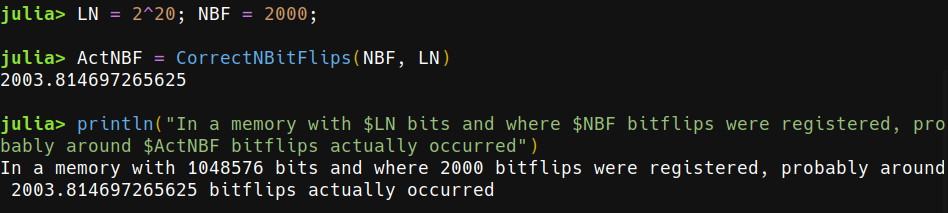
\includegraphics[width=0.75\columnwidth]{fig/functions/CorrectNBitFlips.png}
		\caption{Example of use of \texttt{CorrectNBitFlips}.}
		\label{fig:Example_CorrectNBitflips}
	\end{figure}
	
	Expression is taken from Eq. 6 in F. J. Franco, J. A. Clemente, H. Mecha and R. Velazco, 
	"\textit{Influence of Randomness During the Interpretation of Results From Single-Event Experiments 
		on SRAMs}," IEEE Transactions on Device and Materials Reliability, vol. 19, no. 1, pp. 104-111, 
	March 2019, doi: 10.1109/TDMR.2018.
	2886358.		
\end{itemize}
%
\subsubsection*{NF2BitMCUs}\label{Fun:NF2BitMCUs}
%
\begin{itemize}
	\item \textbf{Input arguments}: 
	\begin{itemize}
		\item \textit{Method 1}: \textbf{NSBU}::Int, \textbf{LA}::Int, \textbf{METHOD}::String, \textbf{D}::Int, \textbf{WordWidth}::Int, \textbf{UsePseudoAddress}::Bool
		\item \textit{Method 2}: \textbf{NSBU}::Int, \textbf{LA}::Int, \textbf{METHOD}::String, \textbf{D}::Int, \textbf{WordWidth}::Int
	\end{itemize}
	\item \textbf{Output}: Float64
	\item It indicates the expected number of false 2-bit MCUs that will occur 
	in a memory with \textbf{LA} words with \textbf{WORDWIDTH} bits each in which \textbf{NSBU} SBUs have occurred. In this analysis, 
	MCUS are sought using some grouping method (\textbf{METHOD}) with a generalized distance \textbf{D}.
	
	If \textbf{UsePseudoAddress} is not provided, its default value is \texttt{false}.
	
	Unlike \hyperref[Fun:NF3BitMCUs]{\texttt{NF3BitMCUs}}, two values are provided as outputs, called  ``\textit{optimistic}'' and ``\textit{pessimistic}''. The actual number of expected false events is somewhere between both values. So far, it is not possible to get  more accurate value, as explained in the theoretical development. Use the values as you may wish.
	
	Admitted values for \textbf{METHOD} and \textbf{D} are the following:
	
	\begin{enumerate}
		\item \textbf{METHOD}: \texttt{"MBU"} \(\rightarrow\) Only MBUs are sought. In this case, \textbf{D} is the \textbf{WORDWiDTH}.
		\item \textbf{METHOD}: \texttt{"MHD"} \(\rightarrow\)  Only possible if the user has been able to place the flipped	cell in the XY plane. Two cells are related if \(\left|x_1-x_2\right|+ \left|y_1-y_2\right|) \le D\). This  is the \textit{``Manhattan distance''}.
		\item \textbf{METHOD}: \texttt{"IND"} \(\rightarrow\)  Only possible if the user has been able to place the flipped	cell in the XY plane. Two cells are related if \(\max(\left|x_1-x_2\right|, \left|y_1-y_2\right|) \le D\). In mathematics, this is the \textit{"infinite distance"}.
		\item \textbf{METHOD}: \texttt{"THD"} \(\rightarrow\)  Only valid if pairs of bitflips are located in a linear bitstream and if the
		distance between cells is smaller than \textbf{D}: \(\left|x_1-x_2\right| \le D\).
		\item \textbf{METHOD}: \texttt{"XOR"}\(\rightarrow\)  Related pairs are got by means of statistical deviations. Addresses are XORed 
		and only if the value is one of the \textbf{D} possible critical values. If the WORD Addresses  
		is used instead of PSEUDOADDRESS, the memory size must be expressed in WORDs, \textbf{LA = LN/WordWidth}.
		IF SO, THE WORDWIDTH MUST BE PROVIDED.
		\item \textbf{METHOD}: \texttt{"POS"}\(\rightarrow\)  Identical to the previous one but with positive subtraction instead of XOR.
	\end{enumerate}
	
	For LELAPE, only the two last methods are of interest. However, the other methods are included in the tool in case you have used another strategy to combine bitflips and wish to know the background noise. Fig. \ref{fig:Example_NF2BitMCUs} is an example of use.
	
	\begin{figure}[h!]
		\centering
		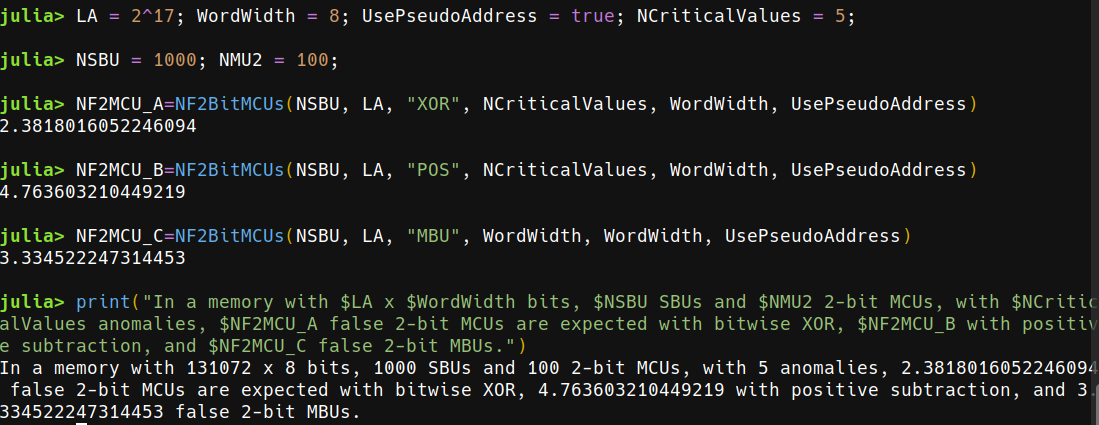
\includegraphics[width=0.75\columnwidth]{fig/functions/NF2BitMCUs.png}
		\caption{Example of use of \texttt{NF2BitMCUs}.}
		\label{fig:Example_NF2BitMCUs}
	\end{figure}	
	
	Everything can be found in Eq. 11 of F. J. Franco, J. A. Clemente, G. Korkian, 
	J. C. Fabero, H. Mecha and R. Velazco, "\textit{Inherent Uncertainty in the Determination of Multiple 
		Event Cross Sections in Radiation Tests,}" IEEE Transactions on Nuclear Science, vol. 67, no. 7, 
	pp. 1547-1554, July 2020, doi: 10.1109/TNS.2020.2977698.
	
\end{itemize}
%
\subsubsection*{NF3BitMCUs}\label{Fun:NF3BitMCUs}
%
\begin{itemize}
	\item \textbf{Input arguments}: 
	\begin{itemize}
		\item \textit{Method 1}: \textbf{NSBU}::Int, \textbf{NMU2}::Int, \textbf{LN}::Int, \textbf{METHOD}::String, \textbf{D}::Int, WordWidth::Int
		\item \textit{Method 2}: \textbf{NSBU}::Int, \textbf{NMU2}::Int, \textbf{LN}::Int, \textbf{METHOD}::String, \textbf{D}::Int
	\end{itemize}
	\item \textbf{Output}: Tuple{Float64, Float64}
	\item     It indicates the expected number of false 3-bit MCUs that will occur 	in a memory with \textbf{LN} bits in which \textbf{NSBU} SBUs and \textbf{NMU2} 2-bit MCUs have occurred. 	In this analysis, MCUS are sought using some grouping method (\textbf{METHOD}) with a generalized 
	distance D.
	
	MCUS are sought using some grouping method (\textbf{METHOD}) with a generalized distance \textbf{D}.
	
	Admitted values for \textbf{METHOD} and \textbf{D} are the following:
	
	\begin{enumerate}
	\item \textbf{METHOD}: \texttt{"MBU"} \(\rightarrow\) Only MBUs are sought. In this case, \textbf{D} is the \textbf{WORDWiDTH}.
	\item \textbf{METHOD}: \texttt{"MHD"} \(\rightarrow\)  Only possible if the user has been able to place the flipped	cell in the XY plane. Two cells are related if \(\left|x_1-x_2\right|+ \left|y_1-y_2\right|) \le D\). This  is the \textit{``Manhattan distance''}.
	\item \textbf{METHOD}: \texttt{"IND"} \(\rightarrow\)  Only possible if the user has been able to place the flipped	cell in the XY plane. Two cells are related if \(\max(\left|x_1-x_2\right|, \left|y_1-y_2\right|) \le D\). In mathematics, this is the \textit{"infinite distance"}.
	\item \textbf{METHOD}: \texttt{"THD"} \(\rightarrow\)  Only valid if pairs of bitflips are located in a linear bitstream and if the
	distance between cells is smaller than \textbf{D}: \(\left|x_1-x_2\right| \le D\).
	\item \textbf{METHOD}: \texttt{"XOR"}\(\rightarrow\)  Related pairs are got by means of statistical deviations. Addresses are XORed 
	and only if the value is one of the \textbf{D} possible critical values. If the WORD Addresses  
	is used instead of PSEUDOADDRESS, the memory size must be expressed in WORDs, \textbf{LA = LN/WordWidth}.
	IF SO, THE WORDWIDTH MUST BE PROVIDED.
	\item \textbf{METHOD}: \texttt{"POs"}\(\rightarrow\)  Identical to the previous one but with positive subtraction instead of XOR.
\end{enumerate}
	
	For LELAPE, only the two last methods are of interest. See Fig. \ref{fig:Example_NF3BitMCUs} for a practical example. However, the other methods are included in the tool in case you have used another strategy to combine bitflips and wish to know the background noise.
	
	\begin{figure}[h!]
		\centering
		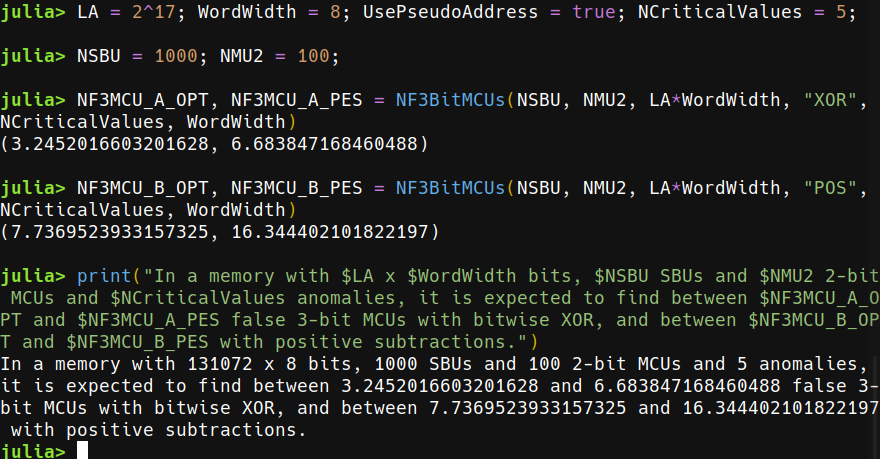
\includegraphics[width=0.75\columnwidth]{fig/functions/NF3BitMCUs.png}
		\caption{Example of use of \texttt{NF3BitMCUs}.}
		\label{fig:Example_NF3BitMCUs}
	\end{figure}	
	
	
	Everything can be found in Eq. 11 of F. J. Franco, J. A. Clemente, G. Korkian, 
	J. C. Fabero, H. Mecha and R. Velazco, "\textit{Inherent Uncertainty in the Determination of Multiple 
		Event Cross Sections in Radiation Tests,}" IEEE Transactions on Nuclear Science, vol. 67, no. 7, 
	pp. 1547-1554, July 2020, doi: 10.1109/TNS.2020.2977698.
	
	In this paper, it was demonstrated that it is mathematically impossible to get an exact value. Therefore,  optimistic and pessimistic results are provided.
\end{itemize}